\documentclass[onepage]{beamer}
\mode<presentation>{
	\setbeamercovered{transparent}
	%\beamertemplatenavigationsymbolsempty
	\setbeamertemplate{footline}[frame number]
% 	\usefonttheme{professionalfonts}
}

% https://tex.stackexchange.com/questions/34166/understanding-minipages-aligning-at-top
\usepackage{adjustbox}

% https://tex.stackexchange.com/questions/124256/how-do-i-get-numbered-entries-in-a-beamer-bibliography
\setbeamertemplate{bibliography item}{\insertbiblabel}

% https://tex.stackexchange.com/questions/49048/how-to-cite-one-bibentry-in-full-length-in-the-body-text
\usepackage{bibentry}
\bibliographystyle{plain}
\nobibliography*
%
% https://tex.stackexchange.com/questions/163827/wrong-vertical-spaces-using-bibentry-within-beamer/163842
\def\mybeamernewblock{%
  \usebeamercolor[fg]{bibliography entry author}%
  \usebeamerfont{bibliography entry author}%
  \usebeamertemplate{bibliography entry author}%
  \def\newblock{%
    \usebeamercolor[fg]{bibliography entry title}%
    \usebeamerfont{bibliography entry title}%
    \usebeamertemplate{bibliography entry title}%
    \def\newblock{%
      \usebeamercolor[fg]{bibliography entry location}%
      \usebeamerfont{bibliography entry location}%
      \usebeamertemplate{bibliography entry location}%
      \def\newblock{%
        \usebeamercolor[fg]{bibliography entry note}%
        \usebeamerfont{bibliography entry note}%
        \usebeamertemplate{bibliography entry note}}}}%
  \leavevmode
}
\newenvironment{references}{\begin{itemize}\let\newblock\mybeamernewblock}{\end{itemize}}


\setbeamersize{text margin left=10pt, text margin right=10pt}
\setbeamertemplate{itemize items}[circle]

\beamertemplatenavigationsymbolsempty

% http://tex.stackexchange.com/questions/8680/how-can-i-insert-a-newline-in-a-framebox
%\usepackage{minibox}
%\usepackage{framed}
%\usepackage[usestackEOL]{stackengine}

% % http://tex.stackexchange.com/questions/167000/annotating-tables-with-tikz-adding-arrows
% \usepackage{color, colortbl}
\usepackage{tikz}
\tikzstyle{every picture}+=[remember picture]
%\usetikzlibrary{tikzmark, positioning, fit, shapes.misc}

%% http://tex.stackexchange.com/questions/91124/itemize-removing-natural-indent
%\usepackage{enumitem}

%% http://tex.stackexchange.com/questions/41408/a-five-level-deep-list
%\usepackage{enumitem}
%\setlistdepth{9}

% https://tex.stackexchange.com/questions/20792/how-to-superimpose-latex-on-a-picture
\usepackage{overpic}

% % http://tex.stackexchange.com/questions/32661/how-to-locate-figures-with-x-y-specified-location-in-a-presentation
% \usepackage[absolute,overlay]{textpos} % absolute positioning of stuff
% \setlength{\TPHorizModule}{1mm}
% \setlength{\TPVertModule}{1mm}

\usepackage{graphicx}
\graphicspath{{../img/}}
\AtBeginDocument{\DeclareGraphicsExtensions{.eps, .png, .gif, .pdf, .jpg}}

\usepackage[makeroom]{cancel}

\usepackage[english]{babel}
\usepackage[T1]{fontenc}
\usepackage{times}

% \usepackage{amssymb}
% \usepackage{nicefrac}
% \usepackage{bbm}
% \usepackage{esint}
% \usepackage{sidecap}

\usepackage{hyperref}
% \hypersetup{pdfpagemode=FullScreen}

\newcommand{\HIDE}[1]{}

\newcommand{\skipline}{{\ }\\}

\newcommand{\EMAIL}{{\color{blue}randreev{\tiny\color{white}.\hspace{-1.5pt}}@{\tiny\color{white}.\hspace{-1.5pt}}stat.sinica.edu.tw}}

\author{\small RA}
\subject{Talks}

\newcommand{\CITE}[1]{{\footnotesize[#1]}}

% \input{definitions}

\providecommand{\DIV}{\mathop{\text{div}}}
\providecommand{\GRAD}{\mathop{\text{grad}}}

\providecommand{\IE}{\mathbb{E}}
\providecommand{\IP}{\mathbb{P}}
\providecommand{\IR}{\mathbb{R}}
\providecommand{\IZ}{\mathbb{Z}}

\providecommand{\duality}[2]{\langle #1 \rangle_{#2}}
\providecommand{\norm}[2]{\| #1 \|_{#2}}
\providecommand{\seminorm}[2]{| #1 |_{#2}}
\providecommand{\VERT}{\ensuremath{| \! | \! |}}
\newcommand{\tnorm}[2]{\VERT{#1}\VERT_{{#2}}}

\newcommand{\cA}{\mathcal{A}}
\newcommand{\cB}{\mathcal{B}}
\newcommand{\cL}{\mathcal{L}}
\newcommand{\cN}{\mathcal{N}}
\newcommand{\cT}{\mathcal{T}}
\newcommand{\cX}{\mathcal{X}}
\newcommand{\cY}{\mathcal{Y}}

\providecommand{\Abf}{\mathbf{A}}
\providecommand{\Bbf}{\mathbf{B}}
\providecommand{\Dbf}{\mathbf{D}}
\providecommand{\Ibf}{\mathbf{I}}
\providecommand{\Jbf}{\mathbf{J}}
\providecommand{\Fbf}{\mathbf{F}}
\providecommand{\Hbf}{\mathbf{H}}
\providecommand{\Mbf}{\mathbf{M}}
\providecommand{\Tbf}{\mathbf{T}}
\providecommand{\Pbf}{\mathbf{P}}
\providecommand{\Vbf}{\mathbf{V}}
\providecommand{\pbf}{\mathbf{p}}
\providecommand{\ubf}{\mathbf{u}}
\providecommand{\vbf}{\mathbf{v}}
\providecommand{\wbf}{\mathbf{w}}
\providecommand{\ybf}{\mathbf{y}}
\providecommand{\zbf}{\mathbf{z}}

\renewcommand{\vec}[1]{\mathbf{#1}}

\providecommand{\T}{\mathsf{T}}

\renewcommand{\hat}[1]{\widehat{#1}}
\renewcommand{\tilde}[1]{\widetilde{#1}}

\newcommand{\rd}{\,\mathrm{d}}

\newcommand{\TEXT}[1]{\quad\text{#1}\quad}

% http://tex.stackexchange.com/questions/211518/beamer-vfill-and-itemize
\def\Bottom#1{\vskip 0pt plus 1filll #1}
\def\BottomRight#1{\Bottom{\hfill #1}}

% MATLAB CODE LISTING
\usepackage{color}
\definecolor{DarkBlue}{rgb}{0,0,0.4}
% \definecolor{DarkRed}{rgb}{0.3,0,0}
\definecolor{DarkGreen}{rgb}{0,0.3,0}
\usepackage{listings}
\lstset{%
	language=MATLAB,
	basicstyle=\bf\ttfamily\tiny,%\footnotesize,
	keywordstyle=\color{DarkBlue},
	numbers=left, numberstyle=\footnotesize, numbersep=4pt,
	commentstyle={\color{DarkGreen}},
% 	backgroundcolor=\color{white},
	showspaces=false, showstringspaces=false, showtabs=false,
	frame=none,
	tabsize=4,
	breaklines=true, breakatwhitespace=false,
	emph={[1]femT_,femT_assemE,femT_assemF,femT_assemFE,femTX_assemLoad,spacetime},
	emphstyle={[1]\color{blue}},
	emph={[2]femX_,femX_MA,femX_b,femX_init,femX_show},
	emphstyle={[2]\color{DarkGreen}},
	morekeywords={parfor,true,false},
	xleftmargin=8pt,
	numbers=none
}


%%%%%%%%%%%%%%%%%%%%%%%%%%%%%%%%%%%%%%%%%%%%%%%%%%%%%%%%%%%%%%%%%%%%%%%%%%%%%%%%
%%
%%%%%%%%%%%%%%%%%%%%%%%%%%%%%%%%%%%%%%%%%%%%%%%%%%%%%%%%%%%%%%%%%%%%%%%%%%%%%%%%

\usepackage{ifthen}

\newcommand{\REDBOX}[1]{
	\setlength{\fboxrule}{1pt}
	\fcolorbox{red}{SeeMeBarely}{$\displaystyle
		#1
	$}
}

\definecolor{SeeMeBarely}{RGB}{230,230,230}
\definecolor{Purple}{RGB}{128,0,128}
\definecolor{DeepPurple}{RGB}{32,0,96}
\newcommand{\ra}[1]{{\color{blue}{#1}}}
\newcommand{\cred}[1]{{\color{red}{#1}}}
\newcommand{\cblu}[1]{{\color{blue}{#1}}}
\newcommand{\cpur}[1]{{\color{Purple}{#1}}}

\DeclareMathOperator*{\argmin}{arg\,min}

\newcommand{\ItemComment}[1]{\hfill{\scriptsize(#1)\normalsize}}


% http://www.webnots.com/vibgyor-rainbow-color-codes/
\definecolor{a}{RGB}{148, 0, 211}
\definecolor{b}{RGB}{75, 0, 130}
\definecolor{c}{RGB}{0, 0, 255}
\definecolor{d}{RGB}{0, 160, 0}
\definecolor{e}{RGB}{200, 200, 0}
\definecolor{f}{RGB}{255, 127, 0}
\definecolor{g}{RGB}{255, 0, 0}
%
\definecolor{z}{RGB}{0, 0, 0}
\definecolor{w}{RGB}{255, 255, 255}

% http://tex.stackexchange.com/questions/17611/how-does-one-type-chinese-in-latex
\usepackage{CJKutf8}
\AtBeginDvi{\input{zhwinfonts}}
%
\newcommand{\REN}{\begin{CJK*}{UTF8}{gbsn}人\end{CJK*}}
\newcommand{\ren}[1]{{\color{#1}\REN}}



%%%%%%%%%%%%%%%%%%%%%%%%%%%%%%%%%%%%%%%%%%%%%%%%%%%%%%%%%%%%%%%%%%%%%%%%%%%%%%%%
\begin{document}
%%%%%%%%%%%%%%%%%%%%%%%%%%%%%%%%%%%%%%%%%%%%%%%%%%%%%%%%%%%%%%%%%%%%%%%%%%%%%%%%
%%%%%%%%%%%%%%%%%%%%%%%%%%%%%%%%%%%%%%%%%%%%%%%%%%%%%%%%%%%%%%%%%%%%%%%%%%%%%%%%

%%%%%%%%%%%%%%%%%%%%%%%%%%%%%%%%%%%%%%%%%%%%%%%%%%%%%%%%%%%%%%%%%%%%%%%%%%%%%%%%
\section{Intro}
%%%%%%%%%%%%%%%%%%%%%%%%%%%%%%%%%%%%%%%%%%%%%%%%%%%%%%%%%%%%%%%%%%%%%%%%%%%%%%%%



\begin{frame}[plain,t]
	\begin{center}
		%\small
		%
		Some stats on the GSE75688 BC dataset
		%
		\\[1\baselineskip]
		\small
		RA
% 		\\[1\baselineskip]
% 		\footnotesize
% 		ISS, AS \\ \EMAIL

		\vspace{1cm}

		%

	\end{center}

	\Bottom{
		\scriptsize
		%Support: 
		\hfill
		Jan 9, 2018
		\\ {\ }
	}
\end{frame}


%%%

% \begin{frame}[t]{DE vs Signal map}{}
% 	\begin{center}
% 		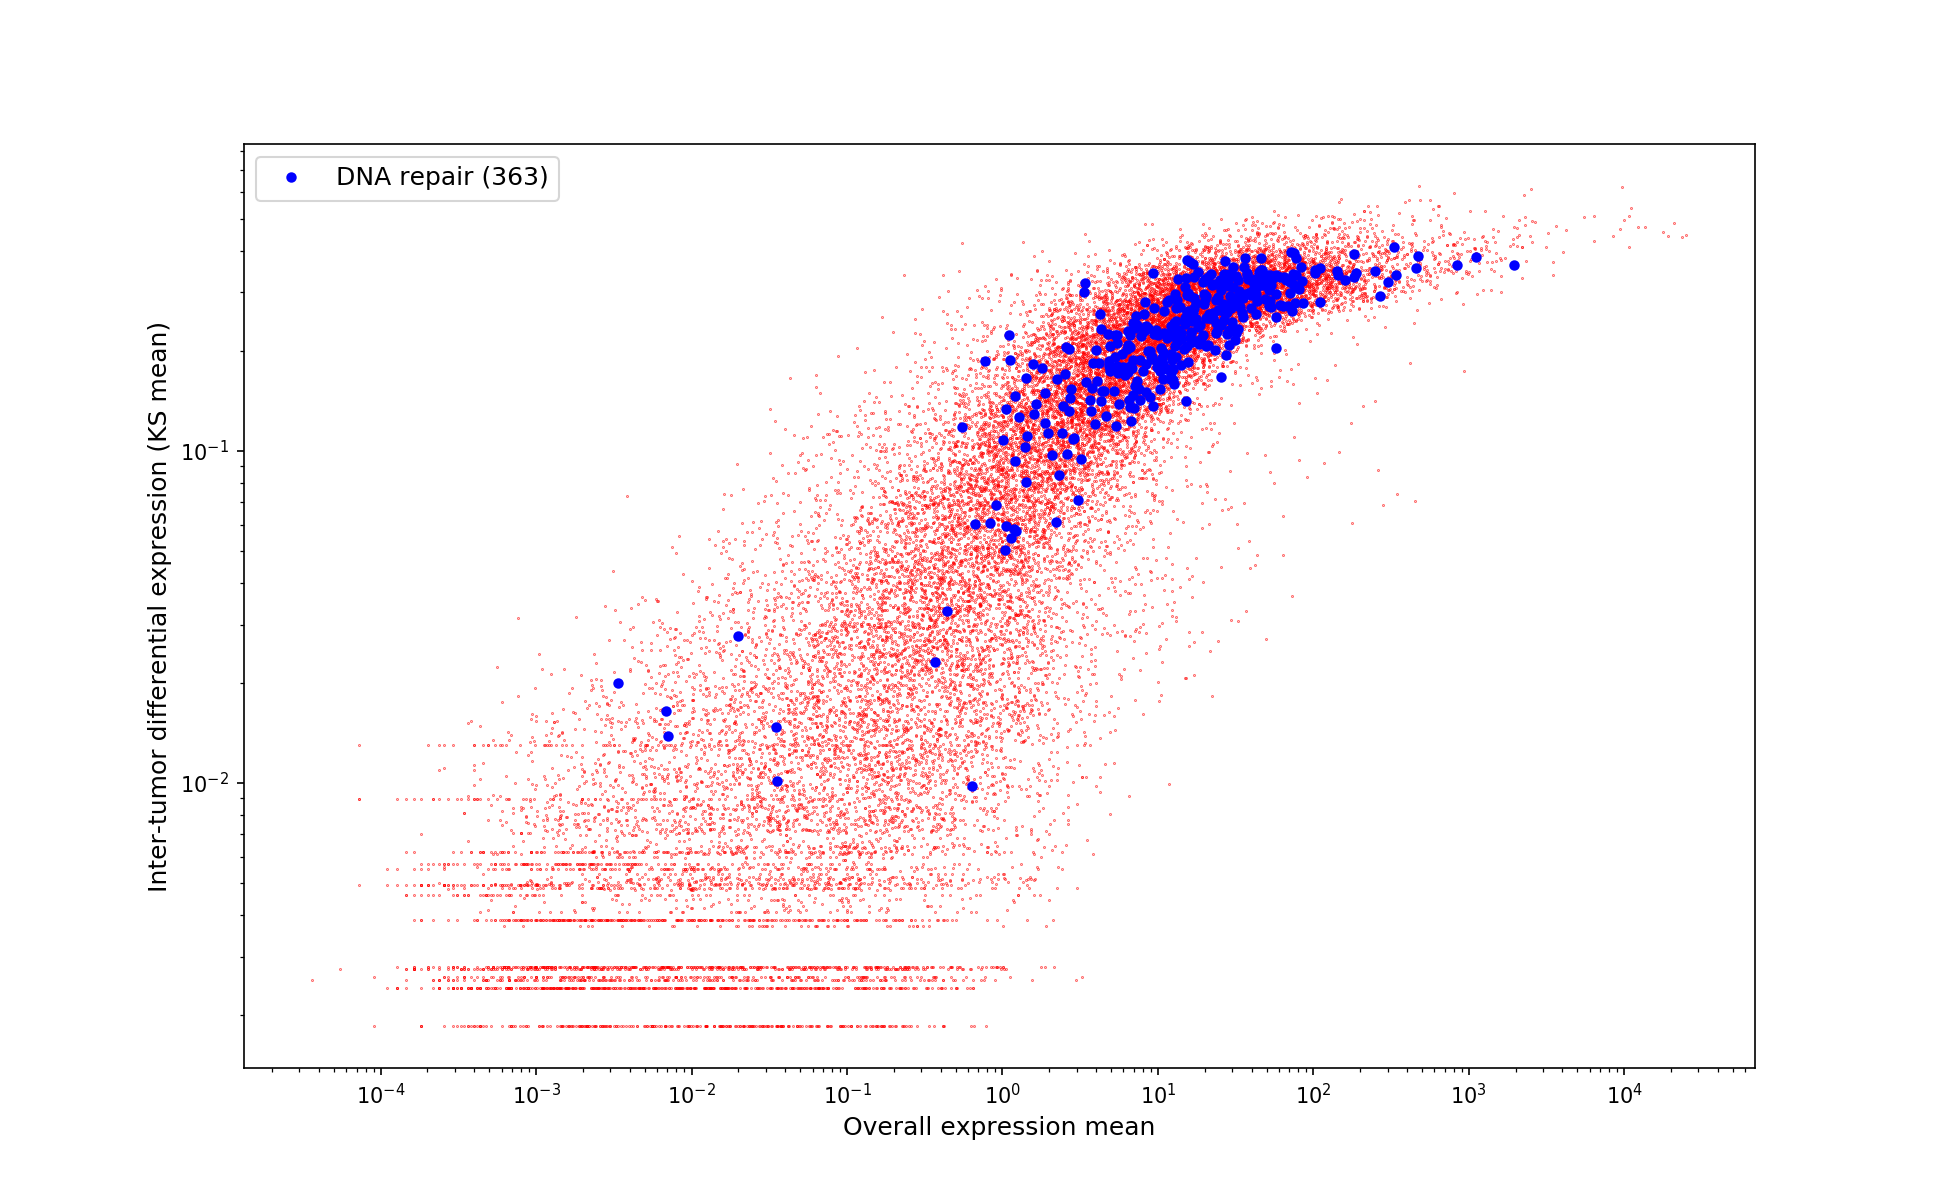
\includegraphics[width=0.99\textwidth]{7_heatmaps/de-vs-ex_GO-0006281}
% 	\end{center}
% 	{\only{GO:0006281 -- DNA repair (363)}}
% \end{frame}

%%%

% \begin{frame}[t]{DE vs Signal map}{Top two DE genes}
% 	\begin{center}
% 		\includegraphics<1>[width=0.99\textwidth]{8_de-vs-ci/de-vs-ex_GO-0006281_log}
% 		\includegraphics<2>[width=0.99\textwidth]{8_de-vs-ci/de-vs-ex_GO-0001525_log}
% 		\includegraphics<3>[width=0.99\textwidth]{8_de-vs-ci/de-vs-ex_GO-0004984_log}
% 		\includegraphics<4>[width=0.99\textwidth]{8_de-vs-ci/de-vs-ex_GO-0006955_log}
% 		\includegraphics<5>[width=0.99\textwidth]{8_de-vs-ci/de-vs-ex_GO-0007049_log}
% 		\includegraphics<6>[width=0.99\textwidth]{8_de-vs-ci/de-vs-ex_GO-0016477_log}
% 	\end{center}
% \end{frame}

%%%

\begin{frame}[t]{Follow-up on Tony's table}{}
	On BC dataset:

	{
		\tiny
		
		\begin{table}[]
		\label{my-label}
		\begin{tabular}{rllll}
			& GO terms                                                               & GO-ID      & NSV Percentage & Gene Numbers \\
		1   & detection of chemical stimulus [in] perception of smell & GO:0050911 & 0.8561020036   & 166          \\
		2   & olfactory receptor activity                                            & GO:0004984 & 0.8561020036   & 166          \\
		3   & antigen binding                                                        & GO:0003823 & 0.7176684882   & 127          \\
		4   & regulation of ion transmembrane transport                              & GO:0034765 & 0.7030965392   & 107          \\
		5   & homophilic cell adhesion via plasma membrane [..]        & GO:0007156 & 0.6921675774   & 146          \\
		6   & calcium ion transmembrane transport                                    & GO:0070588 & 0.6757741348   & 114          \\
		7   & potassium ion transmembrane transport                                  & GO:0071805 & 0.6721311475   & 121          \\
		... &                                                                        &            &                &              \\
		279 & enzyme binding                                                         & GO:0019899 & 0.2987249545   & 319          \\
		280 & negative regulation of transcription, DNA-templated                    & GO:0045892 & 0.2969034608   & 454          \\
		281 & cadherin binding                                                       & GO:0045296 & 0.2969034608   & 277          \\
		282 & protein heterodimerization activity                                    & GO:0046982 & 0.2932604736   & 412          \\
		283 & protein complex                                                        & GO:0043234 & 0.29143898     & 487          \\
		284 & neutrophil degranulation                                               & GO:0043312 & 0.2823315118   & 461         
		\end{tabular}
		\end{table}
	}
	
	{\ }
	
	+ intesection table of 3 datasets.
\end{frame}

%%%

\begin{frame}[t]{Follow-up on Tony's table}{}
	\only<1>{Consistency of GO categories}
	\only<2>{Clustering index: average sign of silhouette values}
	\begin{center}
		\includegraphics<1>[width=0.7\textwidth]{test_txpcompare1/go}
		\includegraphics<2>[width=0.7\textwidth]{test_txpcompare1/ci}
	\end{center}
\end{frame}

%%%

\begin{frame}[t]{Clustering index -- overview}{}
	\begin{center}
		\includegraphics<1>[width=0.99\textwidth]{B_go-by-wq/ci-vs-sz_0}
		\includegraphics<2>[width=0.99\textwidth]{B_go-by-wq/ci-vs-sz_1}
		\includegraphics<3>[width=0.99\textwidth]{B_go-by-wq/ci-vs-sz_2}
		\includegraphics<4>[width=0.99\textwidth]{B_go-by-wq/ci-vs-sz_5}
		\includegraphics<5>[width=0.99\textwidth]{B_go-by-wq/ci-vs-sz_10}
		\includegraphics<6>[width=0.99\textwidth]{B_go-by-wq/ci-vs-sz_90}
		\includegraphics<7>[width=0.99\textwidth]{B_go-by-wq/ci-vs-sz_95}
		\includegraphics<8>[width=0.99\textwidth]{B_go-by-wq/ci-vs-sz_98}
		\includegraphics<9>[width=0.99\textwidth]{B_go-by-wq/ci-vs-sz_99}
	\end{center}
\end{frame}

%%%

\begin{frame}[t]{Clustering index vs Top DE genes}{}
	\begin{center}
		\includegraphics<1>[width=0.99\textwidth]{8_de-vs-ci/ci-vs-de_log_+}
		\includegraphics<2>[width=0.99\textwidth]{8_de-vs-ci/ci-vs-de_log_m}
		\includegraphics<3>[width=0.99\textwidth]{8_de-vs-ci/ci-vs-de_log_r}
		\includegraphics<4>[width=0.99\textwidth]{8_de-vs-ci/ci-vs-de_log_-}
	\end{center}
\end{frame}


%%%

\begin{frame}[t]{}{}
	{\only<1>{Tony's ``Top 50'' from the intersection table:}}
	\begin{center}
		\includegraphics<02>[width=0.99\textwidth]{9_tree/tree_Top50_a}
		\includegraphics<03>[width=0.99\textwidth]{9_tree/tree_Top50_b}
		\includegraphics<04>[width=0.99\textwidth]{9_tree/tree_Top50_c}
		\includegraphics<05>[width=0.99\textwidth]{9_tree/tree_Top50_d}
		\includegraphics<06>[width=0.99\textwidth]{9_tree/tree_Top50_e}
		\includegraphics<07>[width=0.99\textwidth]{9_tree/tree_Top50_f}
		\includegraphics<08>[width=0.99\textwidth]{9_tree/tree_Top50_g}
		\includegraphics<09>[width=0.99\textwidth]{9_tree/tree_Top50_h}
		\includegraphics<10>[width=0.99\textwidth]{9_tree/tree_Top50_i}
		\includegraphics<11>[width=0.99\textwidth]{9_tree/tree_Top50_j}
	\end{center}
\end{frame}

%%%

\begin{frame}[t]{}{}
	{\only<1>{Tony's ``Last 50'' from the intersection table:}}
	\begin{center}
		\includegraphics<02>[width=0.99\textwidth]{9_tree/tree_Last50_a}
		\includegraphics<03>[width=0.99\textwidth]{9_tree/tree_Last50_b}
		\includegraphics<04>[width=0.99\textwidth]{9_tree/tree_Last50_c}
		\includegraphics<05>[width=0.99\textwidth]{9_tree/tree_Last50_d}
		\includegraphics<06>[width=0.99\textwidth]{9_tree/tree_Last50_e}
		\includegraphics<07>[width=0.99\textwidth]{9_tree/tree_Last50_f}
		\includegraphics<08>[width=0.99\textwidth]{9_tree/tree_Last50_g}
		\includegraphics<09>[width=0.99\textwidth]{9_tree/tree_Last50_h}
		\includegraphics<10>[width=0.99\textwidth]{9_tree/tree_Last50_i}
		\includegraphics<11>[width=0.99\textwidth]{9_tree/tree_Last50_j}
		\includegraphics<12>[width=0.99\textwidth]{9_tree/tree_Last50_k}
		\includegraphics<13>[width=0.99\textwidth]{9_tree/tree_Last50_l}
		\includegraphics<14>[width=0.99\textwidth]{9_tree/tree_Last50_m}
		\includegraphics<15>[width=0.99\textwidth]{9_tree/tree_Last50_n}
		\includegraphics<16>[width=0.99\textwidth]{9_tree/tree_Last50_o}
		\includegraphics<17>[width=0.99\textwidth]{9_tree/tree_Last50_p}
		\includegraphics<18>[width=0.99\textwidth]{9_tree/tree_Last50_q}
		\includegraphics<19>[width=0.99\textwidth]{9_tree/tree_Last50_r}
		\includegraphics<20>[width=0.99\textwidth]{9_tree/tree_Last50_s}
		\includegraphics<21>[width=0.99\textwidth]{9_tree/tree_Last50_t}
	\end{center}
\end{frame}

%%%

\begin{frame}[t]{TERT gene}{UniProt O14746, Ensembl \href{http://asia.ensembl.org/Homo_sapiens/Gene/Ontologies/biological_process?g=ENSG00000164362;r=5:1253147-1295069}{ENSG00000164362}}

	\begin{itemize}
	\item
		The best known of the telomere lengthening mechanisms is telomerase [..].
		In contrast to normal somatic tissues, the great majority (ca.~85\%) of human cancers have detectable levels of telomerase [..].

		{\tiny \url{https://www.ncbi.nlm.nih.gov/pmc/articles/PMC4262939/}}
	
	\item
		TERT is expressed only in 5 of 563 samples in the BC dataset:
		
		{
			\tiny
			ENSG00000164362.14 TERT protein-coding 0 ... 0 0.49 0 ... 0 4.24 0 ... 0 2.53 0 ... 0 0.68 0 .... 0 1.19 0 ... 0
		}
	
	\item
		Some immortalized cell lines maintain telomere length for hundreds of population doublings in the absence of telomerase activity, and it was therefore deduced that they must have an alternative lengthening of telomeres (ALT) mechanism.
		
		{\tiny \url{https://www.ncbi.nlm.nih.gov/pmc/articles/PMC4262939/}}
	\end{itemize}

\end{frame}

%%%

\begin{frame}[t]{Telomere maintenance}{}
	\begin{itemize}
	\item
	
		[Up-regulated telomere maintenance mechanisms] and related aspects of telomere structure and function therefore appear to be ideal targets for the development of anticancer therapeutics. 
		
		{\tiny \url{https://www.ncbi.nlm.nih.gov/pmc/articles/PMC4262939/}}
	
	\item
		GO:0097698 (1) -- t.m.\ via base-excision repair
		
		{\only<2>{%
			\begin{itemize}
			\item
				A telomere maintenance process that occurs by base-excision repair of telomeric DNA in response to DNA damage. Telomeric sequences are particularly susceptible to oxidative DNA damage, due to their G-rich nature.
			
				{\tiny \url{http://amigo.geneontology.org/amigo/term/GO:0097698}}
			\item
				Appears in ``GO:0006281 -- DNA repair''
			\end{itemize}
		}}%
	
	\item
		GO:0032201 (24) -- t.m.\ via semi-conservative replication
		
		{\only<3>{%
			\begin{itemize}
			\item
				The process in which telomeric DNA is synthesized semi-conservatively by the conventional replication machinery and telomeric accessory factors as part of cell cycle DNA replication.
			
				{\tiny \url{http://amigo.geneontology.org/amigo/term/GO:0032201}}
			\item
				Appears in ``GO:0006260 -- DNA replication'' with relatively \textbf{low} clustering index
			\end{itemize}
		}}%
	
	\item
		GO:0000723 (40) -- telomere maintenance
		
		{\only<4>{%
			\begin{itemize}
			\item
				Any process that contributes to the maintenance of proper telomeric length and structure by affecting and monitoring the activity of telomeric proteins, the length of telomeric DNA and the replication and repair of the DNA. These processes includes those that shorten, lengthen, replicate and repair the telomeric DNA sequences.
			
				{\tiny \url{http://amigo.geneontology.org/amigo/term/GO:0000723}}
			\end{itemize}
		}}%
	\end{itemize}
\end{frame}

\begin{frame}[t]{}{}
	\begin{center}
		\includegraphics<01>[width=0.99\textwidth]{9_tree/tree_GO-0006281}
		\includegraphics<02>[width=0.99\textwidth]{9_tree/tree_Top50_c}
		\includegraphics<03>[width=0.99\textwidth]{9_tree/tree_GO-0000723}
	\end{center}
\end{frame}

%%%

\begin{frame}[t]{}{}
	Are
	\begin{itemize}
	\item
		GO:0032201 -- t.m.\ via semi-conservative replication
	\item
		GO:0010833 -- t.m.\ via telomere lengthening
		
		\scriptsize
		which is a GO parent of GO:0007004 -- t.m.\ via telomerase
	\end{itemize}
	alternative mechanisms for telomere maintenance?
	
	{\ }
	
	Which mechanism do the cancer cells use?

	{\ }
	
	Note that the two GO categories are disjoint.
\end{frame}

%%%

\begin{frame}[t]{GO:0032201 -- t.m.\ via semi-conservative replication}{}
	\begin{center}
		\includegraphics<01>[width=0.8\textwidth]{7_heatmaps/de-vs-ex_GO-0032201}
		\includegraphics<02>[width=0.8\textwidth]{7_heatmaps/heatmap_GO-0032201}
		\includegraphics<03>[width=0.8\textwidth]{A_followup/clustering_glo_GO-0032201}
		\includegraphics<04>[width=0.8\textwidth]{A_followup/clustering_loc_GO-0032201}
	\end{center}
\end{frame}

%%%

\begin{frame}[t]{GO:0010833 -- t.m.\ via telomere lengthening}{}
	\begin{center}
		\includegraphics<01>[width=0.8\textwidth]{7_heatmaps/de-vs-ex_GO-0010833}
		\includegraphics<02>[width=0.8\textwidth]{7_heatmaps/heatmap_GO-0010833}
		\includegraphics<03>[width=0.8\textwidth]{A_followup/clustering_glo_GO-0010833}
		\includegraphics<04>[width=0.8\textwidth]{A_followup/clustering_loc_GO-0010833}
	\end{center}
\end{frame}

%%%

\begin{frame}[t]{GO vs GO expression comparison}{t.m.\ via t.\ lengthening (GO:0010833) \textbf{vs} t.m.\ via semi-cons.\ repl.\ (GO:0032201)}
	\begin{center}
		\includegraphics<01>[width=0.8\textwidth]{A_followup/cross-go_GO-0032201xGO-0010833_BC01}
		\includegraphics<02>[width=0.8\textwidth]{A_followup/cross-go_GO-0032201xGO-0010833_BC02}
		\includegraphics<03>[width=0.8\textwidth]{A_followup/cross-go_GO-0032201xGO-0010833_BC03}
		\includegraphics<04>[width=0.8\textwidth]{A_followup/cross-go_GO-0032201xGO-0010833_BC03LN}
		\includegraphics<05>[width=0.8\textwidth]{A_followup/cross-go_GO-0032201xGO-0010833_BC04}
		\includegraphics<06>[width=0.8\textwidth]{A_followup/cross-go_GO-0032201xGO-0010833_BC05}
		\includegraphics<07>[width=0.8\textwidth]{A_followup/cross-go_GO-0032201xGO-0010833_BC06}
		\includegraphics<08>[width=0.8\textwidth]{A_followup/cross-go_GO-0032201xGO-0010833_BC07}
		\includegraphics<09>[width=0.8\textwidth]{A_followup/cross-go_GO-0032201xGO-0010833_BC07LN}
		\includegraphics<10>[width=0.8\textwidth]{A_followup/cross-go_GO-0032201xGO-0010833_BC08}
		\includegraphics<11>[width=0.8\textwidth]{A_followup/cross-go_GO-0032201xGO-0010833_BC09}
		\includegraphics<12>[width=0.8\textwidth]{A_followup/cross-go_GO-0032201xGO-0010833_BC09_Re}
		\includegraphics<13>[width=0.8\textwidth]{A_followup/cross-go_GO-0032201xGO-0010833_BC10}
		\includegraphics<14>[width=0.8\textwidth]{A_followup/cross-go_GO-0032201xGO-0010833_BC11}
	\end{center}
\end{frame}

%%%

\begin{frame}[t]{GO vs GO expression comparison}{}
	Alternative solutions for each ``hallmark'' define the subclone identity?

	\begin{center}
		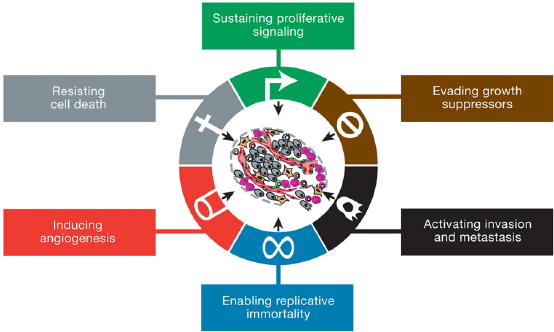
\includegraphics[width=0.7\textwidth]{A_followup/hallmarks}
	\end{center}
	
	{\scriptsize
	[Hallmarks of Cancer: The Next Generation, Hanahan and Weinberg, 2011]
	}
\end{frame}

%%%

\begin{frame}[t]{GO vs GO expression comparison}{}

	On sustaining proliferative signaling
	\begin{itemize}
	\item
		High-throughput DNA sequencing analyses of cancer cell genomes have revealed somatic mutations in certain human tumors that predict constitutive activation of signaling circuits usually triggered by activated growth factor receptors. Thus, we now know that 40\% of human melanomas contain activating mutations affecting the structure of the B-Raf protein, resulting in constitutive signaling through the Raf to \textbf{mitogen-activated protein (MAP)-kinase pathway}. Similarly, mutations in the catalytic subunit of phosphoinositide 3-kinase (PI3-kinase) isoforms are being detected in an array of tumor types, which serve to hyperactivate the \textbf{PI3-kinase signaling} circuitry, including its key Akt/PKB signal transducer.
		
		{\scriptsize
		[Hallmarks of Cancer: The Next Generation, 2011]
		}
	\end{itemize}
\end{frame}

%%%

\begin{frame}[t]{}{}
	Are
	\begin{itemize}
	\item
		GO:0051019 -- MAP kinase binding
	\item
		GO:0035004 -- PI 3-kinase activity
	\end{itemize}
	alternative mechanisms for ``proliferative signaling''?
	
	{\ }
	
	Which mechanism do the cancer cells use?
\end{frame}

%%%

\begin{frame}[t]{GO vs GO expression comparison}{MAP kinase binding (GO:0051019) \textbf{vs} PI 3-kinase activity (GO:0035004)}
	\begin{center}
		\includegraphics<01>[width=0.8\textwidth]{A_followup/cross-go_GO-0035004xGO-0051019_BC01}
		\includegraphics<02>[width=0.8\textwidth]{A_followup/cross-go_GO-0035004xGO-0051019_BC02}
		\includegraphics<03>[width=0.8\textwidth]{A_followup/cross-go_GO-0035004xGO-0051019_BC03}
		\includegraphics<04>[width=0.8\textwidth]{A_followup/cross-go_GO-0035004xGO-0051019_BC03LN}
		\includegraphics<05>[width=0.8\textwidth]{A_followup/cross-go_GO-0035004xGO-0051019_BC04}
		\includegraphics<06>[width=0.8\textwidth]{A_followup/cross-go_GO-0035004xGO-0051019_BC05}
		\includegraphics<07>[width=0.8\textwidth]{A_followup/cross-go_GO-0035004xGO-0051019_BC06}
		\includegraphics<08>[width=0.8\textwidth]{A_followup/cross-go_GO-0035004xGO-0051019_BC07}
		\includegraphics<09>[width=0.8\textwidth]{A_followup/cross-go_GO-0035004xGO-0051019_BC07LN}
		\includegraphics<10>[width=0.8\textwidth]{A_followup/cross-go_GO-0035004xGO-0051019_BC08}
		\includegraphics<11>[width=0.8\textwidth]{A_followup/cross-go_GO-0035004xGO-0051019_BC09}
		\includegraphics<12>[width=0.8\textwidth]{A_followup/cross-go_GO-0035004xGO-0051019_BC09_Re}
		\includegraphics<13>[width=0.8\textwidth]{A_followup/cross-go_GO-0035004xGO-0051019_BC10}
		\includegraphics<14>[width=0.8\textwidth]{A_followup/cross-go_GO-0035004xGO-0051019_BC11}
	\end{center}
\end{frame}

%%%

%%%

%%%

\begin{frame}[t]{Clustering index -- overview}{}
	\begin{center}
		\includegraphics<1>[width=0.99\textwidth]{B_go-by-wq/ci-vs-sz_1}
		\includegraphics<2>[width=0.99\textwidth]{B_go-by-wq/ci-vs-sz_2}
	\end{center}
\end{frame}

%%%

\begin{frame}[t]{GO terms ordered by the windowed quantile}{}
	\begin{table}[]
		\tiny
		\resizebox{\columnwidth}{!}{%
		\begin{tabular}{rlllll}
		      & GO ID      & GO name                                               & Size & Clustering index & CI quantile  \\
		1     & GO:1901339 & regulation of store-operated calcium channel activity & 1    & -0.9958762887    & 0.0001906214 \\
		2     & GO:0005132 & type I interferon receptor binding                    & 6    & -0.9821958457    & 0.0004095004 \\
		3     & GO:0098633 & collagen fibril binding                               & 1    & -0.9954545455    & 0.0004765536 \\
		4     & GO:1904027 & negative regulation of collagen fibril organization   & 1    & -0.9954545455    & 0.0004765536 \\
		5     & GO:0015874 & norepinephrine transport                              & 3    & -0.9875518672    & 0.0005292872 \\
		6     & GO:0005333 & \textbf{norepinephrine transmembrane transporter activity}     & 3    & -0.9875518672    & 0.0005292872 \\
		7     & GO:0008188 & neuropeptide receptor activity                        & 12   & -0.8926174497    & 0.0005382131 \\
		8     & GO:0004956 & prostaglandin D receptor activity                     & 2    & -0.9947089947    & 0.0005512679 \\
		9     & GO:0001785 & prostaglandin J receptor activity                     & 2    & -0.9947089947    & 0.0005512679 \\
		10    & GO:0014050 & negative regulation of glutamate secretion            & 5    & -0.9791122715    & 0.0006347191 \\
		11    & GO:0003837 & beta-ureidopropionase activity                        & 1    & -0.9953488372    & 0.0007624857 \\
		12    & GO:0033038 & bitter taste receptor activity                        & 19   & -0.8965517241    & 0.0007680492 \\
		13    & GO:0005590 & collagen type VII trimer                              & 1    & -0.9951219512    & 0.0009531071 \\
		...   &            &                                                       &      &                  &              \\
		17483 & GO:0070180 & large ribosomal subunit rRNA binding                  & 1    & 0.0544090056     & 1            \\
		17484 & GO:0099503 & secretory vesicle                                     & 3    & -0.4171220401    & 1            \\
		17485 & GO:0030235 & nitric-oxide synthase regulator activity              & 6    & -0.1730418944    & 1            \\
		17486 & GO:0071364 & cellular response to epidermal growth factor stimulus & 40   & 0.1985428051     & 1            \\
		17487 & GO:0016310 & phosphorylation                                       & 679  & 0.7559198543     & 1            \\
		17488 & GO:0016740 & transferase activity                                  & 1717 & 0.8214936248     & 1            \\
		17489 & GO:0016020 & membrane                                              & 7464 & 0.8178506375     & 1           
		\end{tabular}
		}
	\end{table}
\end{frame}

%%%

\begin{frame}[t]{Norepinephrine (noradrenaline)}{GO:0005333 -- norepinephrine transmembrane transporter activity (3)}
	\scriptsize
	
	\begin{itemize}
	\item
		There is growing evidence that the neurotransmitter norepinephrine (NE) and its sister molecule epinephrine (EPI) (adrenaline) affect some types of cancer. \textbf{Several recent epidemiological studies have shown that chronic use of beta blocking drugs (which antagonize NE/EPI receptors) results in lower recurrence, progression, or mortality of breast cancer and malignant melanoma.} Preclinical studies have shown that manipulation of the levels or receptors of NE and EPI with drugs affects experimentally induced cancers. 
		
		[..]
		
		For example, there is growing evidence that NE and adrenoceptors interact with the P38/\textbf{MAPK}, Stat3, and \textbf{PI3K}/AKT signaling pathways. If so, this may provide an additional link between extracellular signaling mechanisms and intracellular signaling pathways, such as P38/MAPK, which are the focus of intensive study by molecular oncology researchers

		{\tiny Clin Epidemiol. 2012; 4: 151--156 (\url{https://www.ncbi.nlm.nih.gov/pmc/articles/PMC3396053/})}
	
	\item
		GO:0005333 contains ENSG00000175003, ENSG00000103546, ENSG00000112499

	\item 
		In the BC dataset:
		
		{
			\tiny
			ENSG00000175003.8 SLC22A1 protein-coding 0 ... 0 0.91 1.01 0 0.6 0 ... 0 0.67 0 0.21 0 ... 0 4.93 0 ... 0 24 0 ... 0 30.95 0 ... 0 0.4 0 ... 0 4.13 0 ... 0 \textbf{51.93} 0 ... 0 \textbf{114.76} 0 ... 0 0.83 0 ... 0 4.82 0 ... 0 1.71 0 ... 0 11.26 0 ... 0 4.49 0 ... 0 1.68 0 ... 0 1.02 0 ... 0 \textbf{83.49} 0 ... 0 11.58 0 ... 0 3.06 1.1 0 ... 0 9.28 0 ... 0 7.82 0 ... 0 3.84 0 ... 0
		}
	\end{itemize}
\end{frame}

\begin{frame}[t]{Norepinephrine (noradrenaline)}{GO:0005333 -- norepinephrine transmembrane transporter activity (3)}
	\begin{center}
		\includegraphics<01>[width=0.8\textwidth]{A_followup/clustering_loc_GO-0005333}
	\end{center}
\end{frame}

%%%%%%%%%%%%%%%%%%%%%%%%%%%%%%%%%%%%%%%%%%%%%%%%%%%%%%%%%%%%%%%%%%%%%%%%%%%%%%%%%
%\section{Extra}
%%%%%%%%%%%%%%%%%%%%%%%%%%%%%%%%%%%%%%%%%%%%%%%%%%%%%%%%%%%%%%%%%%%%%%%%%%%%%%%%%
%
%
\newcounter{finalframe}
\setcounter{finalframe}{\value{framenumber}}
% Backup frames follow
%
%
%\begin{frame}
%	Appendix
%\end{frame}
%
%%
%
%\begin{frame}
%	%
%\end{frame}
%
%
% FINAL SLIDE
\setbeamercolor{background canvas}{bg=black}
\begin{frame}[plain,b]
	\hfill
	\tiny
	\color{gray}
	this slide is intentionally left blank
\end{frame}
\setbeamercolor{background canvas}{bg=white}


%%%%%%%%%%%%%%%%%%%%%%%%%%%%%%%%%%%%%%%%%%%%%%%%%%%%%%%%%%%%%%%%%%%%%%%%%%%%%%%%%
%\section{Bibliography}
%%%%%%%%%%%%%%%%%%%%%%%%%%%%%%%%%%%%%%%%%%%%%%%%%%%%%%%%%%%%%%%%%%%%%%%%%%%%%%%%%

% {
% \tiny
% \bibliography{../../../r/refs}
% }


%%%%%%%%%%%%%%%%%%%%%%%%%%%%%%%%%%%%%%%%%%%%%%%%%%%%%%%%%%%%%%%%%%%%%%%%%%%%%%%%
\setcounter{framenumber}{\value{finalframe}}
\end{document}
%%%%%%%%%%%%%%%%%%%%%%%%%%%%%%%%%%%%%%%%%%%%%%%%%%%%%%%%%%%%%%%%%%%%%%%%%%%%%%%%
%%%%%%%%%%%%%%%%%%%%%%%%%%%%%%%%%%%%%%%%%%%%%%%%%%%%%%%%%%%%%%%%%%%%%%%%%%%%%%%%

